\documentclass{beamer}
\usetheme{CambridgeUS}

%----macros begin-----------------------------------------------------------------------------------
\usepackage{graphicx}
\usepackage{color}
\usepackage{xcolor}
\usepackage{amsfonts}
\usepackage{amsmath}
%\usepackage{amsthm}
%\usepackage[utf8]{inputenc}
\usepackage{framed}
\usepackage{wasysym}

\newcommand{\columnsbegin}{\begin{columns}}
\newcommand{\columnsend}{\end{columns}}

%\renewenvironment{Shaded}{\pause\begin{snugshade}}{\end{snugshade}}
\def\twocolumns#1#2{\begin{columns}
\begin{column}{0.5\linewidth}#1\end{column}
\begin{column}{0.5\linewidth}#2\end{column}
\end{columns}}
\def\mytwocolumns#1#2#3#4{\begin{columns}
\begin{column}{#1\linewidth}#2\end{column}
\begin{column}{#3\linewidth}#4\end{column}
\end{columns}}
\def\mythreecolumns#1#2#3#4#5#6{\begin{columns}
\begin{column}{#1\linewidth}#2\end{column}
\begin{column}{#3\linewidth}#4\end{column}
\begin{column}{#5\linewidth}#6\end{column}
\end{columns}}
\def\threecolumns#1#2#3{\begin{columns}
\begin{column}{0.33\linewidth}#1\end{column}
\begin{column}{0.33\linewidth}#2\end{column}
\begin{column}{0.33\linewidth}#3\end{column}
\end{columns}}
\def\fourcolumns#1#2#3#4{\begin{columns}%
\begin{column}{0.25\linewidth}#1\end{column}%
\begin{column}{0.25\linewidth}#2\end{column}%
\begin{column}{0.25\linewidth}#3\end{column}%
\begin{column}{0.25\linewidth}#4\end{column}%
\end{columns}}

\def\textbf#1{\alert{#1}}
\def\emph#1{{\color{cyan}#1}}
\def\conv{\mbox{\textrm{conv}\,}}
\def\aff{\mbox{\textrm{aff}\,}}
\def\E{\mathbb{E}}
\def\R{\mathbb{R}}
\def\Z{\mathbb{Z}}
\def\N{\mathbb{N}}
\def\P{\mathbb{P}}
\def\v#1{{\bf #1}}
\def\p#1{{\bf #1}}
\def\T#1{{\bf #1}}
\def\vet#1{{\left(\begin{array}{cccccccccccccccccccc}#1\end{array}\right)}}
\def\mat#1{{\left(\begin{array}{cccccccccccccccccccccccccccc}#1\end{array}\right)}}

\def\lin{\mbox{\rm lin}\,}
\def\aff{\mbox{\rm aff}\,}
\def\pos{\mbox{\rm pos}\,}
\def\cone{\mbox{\rm cone}\,}
\def\conv{\mbox{\rm conv}\,}
\newcommand{\homog}[0]{\mbox{\rm homog}\,}
\newcommand{\relint}[0]{\mbox{\rm relint}\,}

\newtheorem{assignment}{Assignment}
\newtheorem{exercise}{Exercise}
\newtheorem{question}{Question}
\newtheorem{remark}{Remark}
%----macros end-----------------------------------------------------------------------------------

\newcommand\myenum[1]{% 
  \begin{pgfpicture}{-1ex}{-0.65ex}{1ex}{1ex} 
    \usebeamercolor[fg]{item projected} 
    {\pgftransformscale{1.75}\pgftext{\normalsize\pgfuseshading{bigsphere}}} 
    {\pgftransformshift{\pgfpoint{0pt}{0.5pt}} 
      \pgftext{\usebeamerfont*{item projected}#1}} 
  \end{pgfpicture}% 
} 

\definecolor{whitesmoke}{HTML}{F5F5F5}

%
%\usepackage{listings}
%\lstdefinestyle{bash-style}{
%  captionpos=b,
%  belowcaptionskip=1\baselineskip,
%  breaklines=true,
%  tabsize=2,
%  frame=tb,
%  aboveskip=3mm,
%  belowskip=3mm,
%  xleftmargin=\parindent,
%  language=bash,
%  showstringspaces=false,
%  % basicstyle=\tiny, %\footnotesize\ttfamily,
%  basicstyle={\fontsize{8pt}{8pt}\ttfamily},
%  keywordstyle=\color{black},
%  commentstyle=\color{green!40!black},
%  stringstyle=\color{brown},
%  identifierstyle=\color{black},
%  backgroundcolor=\color{whitesmoke}
%}
%\lstdefinestyle{python-style}{
%  captionpos=b,
%  belowcaptionskip=1\baselineskip,
%  breaklines=true,
%  tabsize=2,
%  frame=tb,
%  aboveskip=3mm,
%  belowskip=3mm,
%  xleftmargin=\parindent,
%  language=Python,
%  showstringspaces=false,
%  % basicstyle=\tiny, %\footnotesize\ttfamily,
%  basicstyle={\fontsize{8pt}{8pt}\ttfamily},
%  keywordstyle=\color{blue},
%  commentstyle=\color{green!40!black},
%  stringstyle=\color{brown},
%  identifierstyle=\color{blue},
%  backgroundcolor=\color{whitesmoke}
%}


% Default fixed font does not support bold face
\DeclareFixedFont{\ttb}{T1}{txtt}{bx}{n}{12} % for bold
\DeclareFixedFont{\ttm}{T1}{txtt}{m}{n}{12}  % for normal

% Custom colors
\usepackage{color}
\definecolor{deepblue}{rgb}{0,0,0.5}
\definecolor{deepred}{rgb}{0.6,0,0}
\definecolor{deepgreen}{rgb}{0,0.5,0}
\definecolor{whitesmoke}{HTML}{F5F5F5}

\usepackage{listings}

% Python style for highlighting
\newcommand\pythonstyle{\lstset{
language=Python,
basicstyle=\ttm,
otherkeywords={self},             % Add keywords here
keywordstyle=\ttb\color{orange},
emph={MyClass,__init__},          % Custom highlighting
emphstyle=\ttb\color{deepred},    % Custom highlighting style
stringstyle=\color{deepgreen},
frame=tb,                         % Any extra options here
showstringspaces=false,           % 
  captionpos=b,
  belowcaptionskip=1\baselineskip,
  breaklines=true,
  tabsize=2,
  frame=tb,
  aboveskip=3mm,
  belowskip=3mm,
  xleftmargin=\parindent,
  language=Python,
  showstringspaces=false,
  basicstyle=\footnotesize\ttfamily,
  basicstyle={\fontsize{8pt}{8pt}\ttfamily},
  % keywordstyle=\color{blue},
  commentstyle=\color{deepgreen}\slshape,
  stringstyle=\color{brown},
  identifierstyle=\color{blue},
% language=python,
% basicstyle=\ttfamily\scriptsize\setstretch{1},
% stringstyle=\color{red},
% showstringspaces=false,
% alsoletter={1234567890},
% otherkeywords={\ , \}, \{},
% keywordstyle=\color{blue},
emph={access,and,break,class,continue,def,del,elif ,else,%
except,exec,finally,for,from,global,if,import,in,i s,%
lambda,not,or,pass,print,raise,return,try,while},
emphstyle=\color{black}\bfseries,
emph={[2]True, False, None, self},
emphstyle=[2]\color{green},
emph={[3]from, import, as},
emphstyle=[3]\color{red},
upquote=true,
morecomment=[s]{"""}{"""},
%commentstyle=\color{gray}\slshape,
emph={[4]1, 2, 3, 4, 5, 6, 7, 8, 9, 0},
% emphstyle=[4]\color{blue},
%literate=*{:}{{\textcolor{blue}:}}{1}%
%{=}{{\textcolor{blue}=}}{1}%
%{-}{{\textcolor{blue}-}}{1}%
%{+}{{\textcolor{blue}+}}{1}%
%{*}{{\textcolor{blue}*}}{1}%
%{!}{{\textcolor{blue}!}}{1}%
%{(}{{\textcolor{blue}(}}{1}%
%{)}{{\textcolor{blue})}}{1}%
%{[}{{\textcolor{blue}[}}{1}%
%{]}{{\textcolor{blue}]}}{1}%
%{<}{{\textcolor{blue}<}}{1}%
%{>}{{\textcolor{blue}>}}{1},%  
  backgroundcolor=\color{whitesmoke}
}}


% Python environment
\lstnewenvironment{python}[1][]
{
\pythonstyle
\lstset{#1}
}
{}

% Python for external files
\newcommand\pythonexternal[2][]{{
\pythonstyle
\lstinputlisting[#1]{#2}}}

% Python for inline
\newcommand\pythoninline[1]{{\pythonstyle\lstinline!#1!}}



% \usepackage{beamerthemesplit} // Activate for custom appearance


\title{Geometric \& Graphics Programming Lab: Lecture 9}
\author{Alberto Paoluzzi}
\date{\today}

\nonstopmode



\begin{document}

\frame{\titlepage}

\section[Outline]{}
\frame{\tableofcontents}


%---------------------------------------------------------------------- SLIDE -

\section{3D Affine transformations}

%---------------------------------------------------------------------- SLIDE -
\begin{frame}\frametitle{Introduction}

\vfill


A 3D extension of plane \emph{translation and scaling} is easy

\vfill

A major care is only needed for \emph{3D rotation} and \emph{3D shearing}

\vfill

In order to unify the tratment of linear and affine transformations, and to use the \emph{matrix product} as the only geometric operator,  we use \emph{normalized homogeneous coordinates} and tensors in \emph{$\lin\ \R^4$} 

\vfill
\end{frame}
%---------------------------------------------------------------------- SLIDE -
\subsection{Translation and scaling}
%---------------------------------------------------------------------- SLIDE -
\begin{frame}\frametitle{Translation}

\vfill

\alert{Translation} tensor $\T{T}_{xyz}(l,m,n)$ with parameters $l, m, n$ (the components of the translation vector), and its matrix:

\vfill

\[
\T{T}_{xyz}(l,m,n) =
\mat{
1 & 0 & 0 & l\\
0 & 1 & 0 & m\\
0 & 0 & 1 & n\\
0 & 0 & 0 & 1
}\]

\vfill


\begin{remark}
Here the homogeneous row and column are the last ones !!
\end{remark}

\end{frame}
%---------------------------------------------------------------------- SLIDE -
\begin{frame}[fragile]
\frametitle{Translation}
\framesubtitle{Predefined operator in \texttt{Pyplasm}}


\vfill

\centering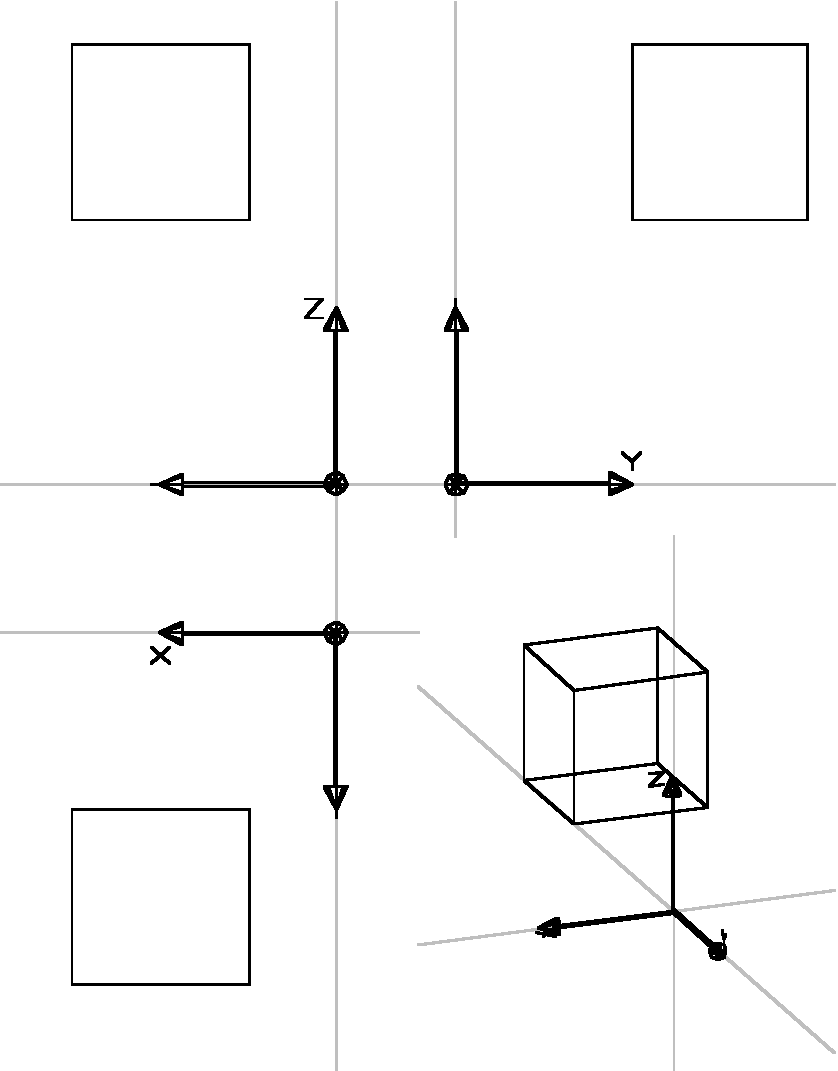
\includegraphics[width=0.4\linewidth]{figs/cube-t}

\vfill

\begin{python}
  T([1,2,3])([0.5,1,1.5])(CUBOID([1,1,1]))
\end{python}


\end{frame}
%---------------------------------------------------------------------- SLIDE -
\begin{frame}\frametitle{Scaling}

\vfill

The  \emph{scaling} tensor $\T{S}_{xyz}(a,b,c)$ with parameters  $a, b, c$ is represented in coordinates by the matrix
\vfill

\[\T{S}_{xyz}(a,b,c) =
\mat{
a & 0 & 0 & 0\\
0 & b & 0 & 0\\
0 & 0 & c & 0\\
0 & 0 & 0 & 1
}.
\]

\vfill
\end{frame}
%---------------------------------------------------------------------- SLIDE -
\begin{frame}[fragile]
\frametitle{Scaling}
\framesubtitle{Predefined operator in \texttt{Pyplasm}}

    
\vfill

\centering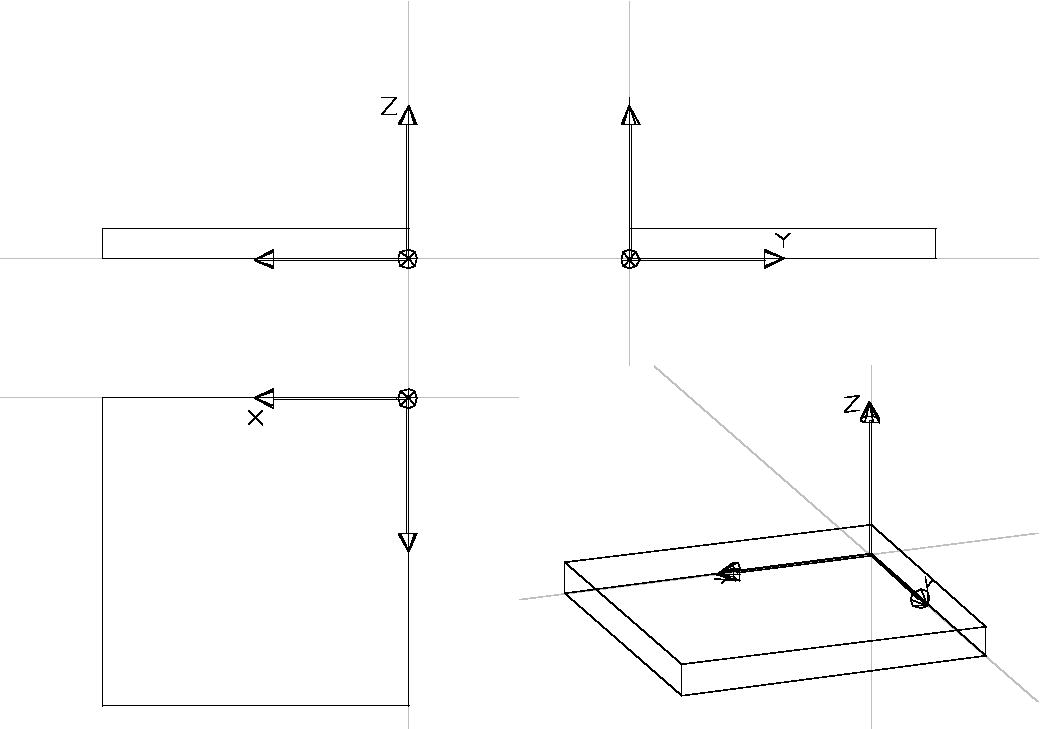
\includegraphics[width=0.7\linewidth]{figs/cube-s}


\vfill

\begin{python}
  S([1,2,3])([2,2,0.2])(CUBOID([1,1,1]))
\end{python}


\end{frame}
%---------------------------------------------------------------------- SLIDE -
\subsection{Rotation}
%---------------------------------------------------------------------- SLIDE -
\begin{frame}\frametitle{Elementary rotations}\small
\framesubtitle{There are ${d}\choose{2}$ different elementary rotations in $\E^d$}

\vfill

Given a Cartesian frame in $\E^{3}$, we call  \emph{elementary rotations} $\T{R}_{yz}$,$\T{R}_{xz}$ and $\T{R}_{xy}$, three functions $\R\rightarrow\lin \R^{3}$, which give, for every angle, the rotation tensor about a cooordinate axis

\vfill

\[
%\T{R}_{yz}(\alpha) =
\mat{
1 & 0 & 0 \\
0 & \cos\alpha & -\sin\alpha \\
0 & \sin\alpha & \cos\alpha 
},\
%\T{R}_{xz}(\beta) =
\mat{
\cos\beta & 0 & \sin\beta \\
0 & 1 & 0 \\
-\sin\beta & 0 & \cos\beta 
},\
%\T{R}_{xy}(\gamma) =
\mat{
\cos\gamma & -\sin\gamma & 0 \\
\sin\gamma & \cos\gamma & 0 \\
0 & 0 & 1 
}.
\]
\vfill\centering

Matrices in Cartesian coordinates 

\end{frame}
%---------------------------------------------------------------------- SLIDE -
\begin{frame}[fragile]
\frametitle{Elementary rotations}
\framesubtitle{Predefined operator in \texttt{Pyplasm}}


\vfill

\centering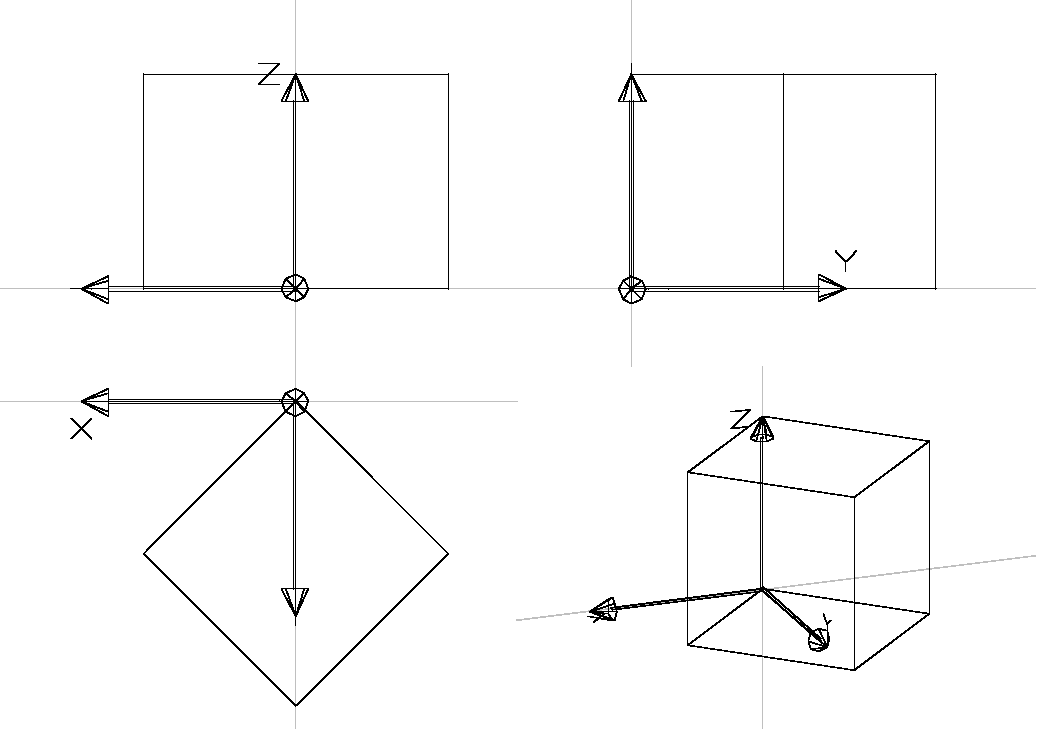
\includegraphics[width=0.6\linewidth]{figs/cube-r}


\vfill

\begin{python}
  R([1,2])(PI/4)(CUBOID([1,1,1]))
\end{python}


\end{frame}
%---------------------------------------------------------------------- SLIDE -
\begin{frame}[fragile]
\frametitle{Elementary rotations}
\framesubtitle{example}\small


Here we define a parallelepiped  \texttt{element},  translated  in $x,y$ by a tensor \texttt{T([1,2])([-5,-5])} to move its center upon the $z$ axis

\vfill

\centering{
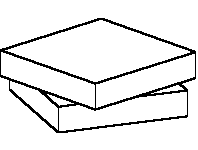
\includegraphics[width=1.2cm]{figs/rotBox0}
\hspace{2cm}
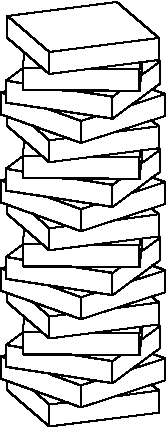
\includegraphics[width=1.2cm]{figs/rotBox1}
}

\vfill

\begin{python}
element = COMP([T([1,2])([-5,-5]), CUBOID])([10,10,2])
element = T([1,2])([-5,-5])( CUBOID([10,10,2]) )

column = STRUCT( NN(17)([element, T(3)(2), R([1,2])(PI/8)]) )
column = STRUCT( CAT(N(17)([element, T(3)(2), R([1,2])(PI/8)])) )

VIEW(column)
\end{python}
equivalent expressions

\vfill
\end{frame}
%---------------------------------------------------------------------- SLIDE -
\begin{frame}\frametitle{General rotation}\small

\vfill

A rotation of $\E^3$ is a linear orthogonal transformation with a set of fixed points (\emph{eigenspace} in linear algebra) of dimension~$1$, known as \emph{rotation axis}

\vfill
In this transformation, every point (not on the axis) is mapped in the other extreme of a circumference arc of constant angle, centered on the axis, and contained in a plane orthogonal to it.
\vfill

We will compute the rotation matrix of the tensor
$\T{R}_{xyz}(\v{n}, \alpha)$, with

\[
\T{R}_{xyz} : \R^{3}\times\R \rightarrow \lin\R^{4} :
(\v{n}, \alpha) \mapsto \T{R}_{xyz}(\v{n}, \alpha),
\]

where the vector $\v{n}$ is parallel to the rotation axis, and $\alpha$ is the angle of rotation
\vfill
\end{frame}
%---------------------------------------------------------------------- SLIDE -
\begin{frame}
\frametitle{General rotation}
\framesubtitle{by composition of elementary rotations}\small

A 3D non elementary rotation $\T{R}_{xyz}(\v{n}, \alpha)$, with axis $n$ and $\alpha$ angle, can be reduced to the composition of elementary rotations:

\vfill

\begin{eqnarray*}
\T{R}_{xyz}(\v{n}, \alpha)
&=&
(\T{R}_y(\gamma)\circ \T{R}_x(\beta))^{-1}\circ
\T{R}_z(\alpha)\circ
(\T{R}_y(\gamma)\circ \T{R}_x(\beta)) \\[0.3cm] \hfill
&=&
\T{R}_x(\beta)^{-1}\circ \T{R}_y(\gamma)^{-1}\circ
\T{R}_z(\alpha)\circ
\T{R}_y(\gamma)\circ \T{R}_x(\beta) \\[0.3cm] \hfill
&=&
\T{R}_x(-\beta)\circ \T{R}_y(-\gamma)\circ
\T{R}_z(\alpha)\circ
\T{R}_y(\gamma)\circ \T{R}_x(\beta) .
\end{eqnarray*}


\end{frame}
%---------------------------------------------------------------------- SLIDE -
\begin{frame}
\frametitle{General rotation}
\framesubtitle{by composition of elementary rotations}\small

\vfill
\begin{center}
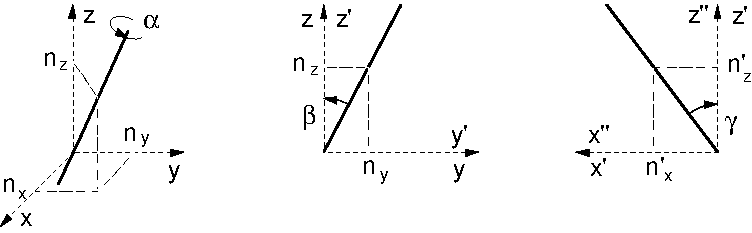
\includegraphics[width=\linewidth]{figs/rotelem}

(a)~~$\v{n}$ axis; (b) rotation about $x$; (c) rotation about $y$
\end{center}
\vfill
\[
\beta = \arctan\left({n_y\over n_z}\right)
\qquad
\gamma = -\arctan\left({n'_x\over n'_z}\right)
\]
where $\v{n}' = \T{R}_x(\beta)\  \v{n}$.


\end{frame}
%---------------------------------------------------------------------- SLIDE -
\begin{frame}
\frametitle{General rotation}
\framesubtitle{by transformation of coordinates}\small

The tensor  $\T{R}_{xyz}(\v{n}, \alpha)$ of a general rotation may be computed by composition of three tensors:

\vfill

\[
\T{R}_{xyz}(\v{n}, \alpha) =
\T{Q}^{-1}_{{\scriptsize \v{n}}}\circ \T{R}_z(\alpha)\circ \T{Q}_{{\scriptsize \v{n}}}.
\]

\vfill

such that:

\vfill

\begin{enumerate}
\item
a coordinate transformation $\T{Q}_{{\scriptsize \v{n}}}$ that maps the unit vector $\v{n}\over |\v{n}|$ and two orthogonal versors to the elements of a new basis;

\item\vspace{-2mm}
a rotation $\T{R}_{z}(\alpha)$ about the $z$ axis of this new basis;

\item\vspace{-2mm}
the inverse coordinate transformation $\T{Q}^{-1}_{{\scriptsize \v{n}}}$.
\end{enumerate}
\vfill
\end{frame}
%---------------------------------------------------------------------- SLIDE -
\begin{frame}
\frametitle{General rotation}
\framesubtitle{by transformation of coordinates}\small

We choose a \emph{triple} $\v{q}_x, \v{q}_y, \v{q}_z$ of \emph{orthonormal vectors},  with an element oriented as the rotation axis
\vfill

such vectors are mapped to the basis $\{{\v{e}}_i\}$ by the \emph{unknown matrix} $\T{Q}_{{\scriptsize \v{n}}}$:
\[
\mat{
{\v{e}}_1 & {\v{e}}_2 & {\v{e}}_3
}
=
\T{Q}_{{\scriptsize \v{n}}}\
\mat{
\v{q}_x & \v{q}_y & \v{q}_z
}.
\]

so that

\[
\T{Q}_{{\scriptsize \v{n}}} = \mat{
\v{q}_x & \v{q}_y & \v{q}_z
}^{-1}
= \mat{
\v{q}_x & \v{q}_y & \v{q}_z
}^T
= \mat{
\v{q}_x^T \\ \v{q}_y^T \\ \v{q}_z^T
}
\]
\end{frame}
%---------------------------------------------------------------------- SLIDE -
\begin{frame}
\frametitle{General rotation}
\framesubtitle{by transformation of coordinates}\small

Let us start by setting

\[
\v{q}_z = {\v{n}\over |\v{n}|},
\]

\vfill

We suppose that  $\v{n}\not=\v{e}_3$ is verified --- if false, it would imply $\T{R}(\v{n}, \alpha) =
\T{R}_z(\alpha)$. 

\vfill

Therefore:

\vfill

\[
\v{q}_x = {{\v{e}_3 \times \v{n}}\over |{\v{e}_3 \times \v{n}}|},
\qquad\mbox{and}\qquad
\v{q}_y = {\v{q}_z\times \v{q}_x}.
\]

\end{frame}
%---------------------------------------------------------------------- SLIDE -
\begin{frame}[fragile]
\frametitle{General rotation}
\framesubtitle{Implementation by transformation of coordinates}\small



\vfill

\begin{python}
def ROTN (args):
	""" computation of a general rotation tensor in 3D """
    alpha, n = args
    n  = UNITVECT(n)
    qx = UNITVECT((VECTPROD([[0,0,1], n])))
    qz = UNITVECT(n)
    qy = VECTPROD([qz,qx])
    Q  = MATHOM([qx, qy, qz])
    if n[0]==0 and n[1]==0:
        return R([1, 2])(alpha)
    else:
        return COMP([MAT(TRANS(Q)),R([1,2])(alpha),MAT(Q)])

VIEW( ROTN([PI/4, [0,0,1]])(CUBE(1)) )
VIEW( ROTN([PI/4, [1,1,1]])(CUBE(1)) )
\end{python}


\end{frame}
%---------------------------------------------------------------------- SLIDE -
\begin{frame}[fragile]
\frametitle{General rotation}
\framesubtitle{example}\small

\centering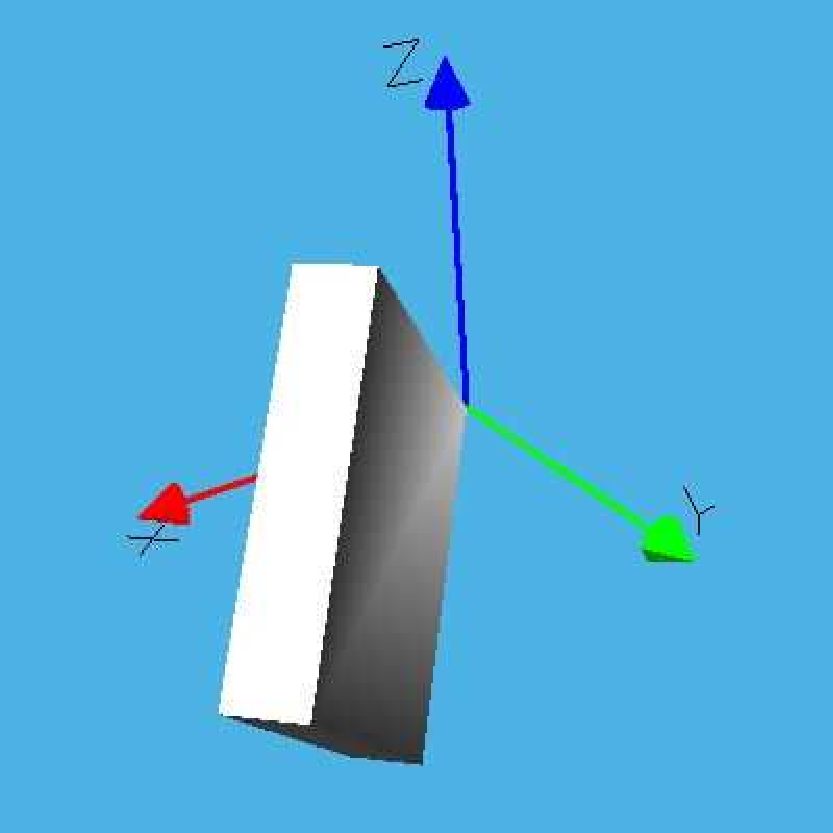
\includegraphics[width=0.4\linewidth]{figs/mkframe}

\vfill

\begin{python}
obj = ROTN([ pi/2, [1,1,0] ])(CUBOID([1,1,0.2]))
VIEW(obj)
\end{python}

\end{frame}

%---------------------------------------------------------------------- SLIDE -
\subsection{Shearing}
%---------------------------------------------------------------------- SLIDE -
\begin{frame}\frametitle{Elementary shearing}\small

A 3D \emph{elementary shearing}  is a tensor that does'nt change one coordinate of $\E^3$ points, and maps the others as linear functions of the non-transformed coordinate 

\vfill

We may distinguish three elementary shearing tensors $\T{H}_{yz}(a,b)$, $\T{H}_{xz}(a,b)$ and
$\T{H}_{xy}(a,b)$, whose matrices differ from the identity only by the elements of a single column

\vfill
\[
%\T{H}_{yz}(a,b) =
\mat{
1 & 0 & 0 & 0\\
a & 1 & 0 & 0\\
b & 0 & 1 & 0\\
0 & 0 & 0 & 1
}, \quad
%\T{H}_{xz}(a,b) =
\mat{
1 & a & 0 & 0\\
0 & 1 & 0 & 0\\
0 & b & 1 & 0\\
0 & 0 & 0 & 1
}, \quad
%\T{H}_{xy}(a,b) =
\mat{
1 & 0 & a & 0\\
0 & 1 & b & 0\\
0 & 0 & 1 & 0\\
0 & 0 & 0 & 1
}
\]

\end{frame}
%---------------------------------------------------------------------- SLIDE -
\begin{frame}\frametitle{Elementary shearing}\small

\begin{itemize}
\item Let consider the 3D space as a bundle of planes parallel to a coordinate plane, that remains fixed 
\item The other planes are translated on theirselves, by a linear function of their distance from the fixed plane 
\end{itemize}


\begin{eqnarray*}
\p{p}^* &=& \T{H}_x(a,b)\ \p{p}  = (x,\  y + ax,\  z + bx,\  1)^T\\
\p{p}^* &=& \T{H}_y(a,b)\ \p{p}  = (x + ay,\  y,\  z + by,\ 1)^T\\
\p{p}^* &=& \T{H}_z(a,b)\ \p{p}  = (x+ az,\ y + bz,\  z,\  1)^T
\end{eqnarray*}

\vfill

with respect to the tensor $\T{H}_z=\T{H}_{xy}(a,b)$:

\begin{enumerate}
    \item
    the $z=0$ plane is invariant;

    \item\vspace{-2mm}
    the $z=1$ plane translates by the translation vector
    $\v{t}=(a,b,0)^{T}$;

    \item\vspace{-2mm}
    each plane $z=c$ translates by a vector $\v{t}'= c (a,b,0)^{T}$.
\end{enumerate}


\end{frame}
%---------------------------------------------------------------------- SLIDE -
%---------------------------------------------------------------------- SLIDE -
\begin{frame}[fragile]
\frametitle{Elementary shearing \hfill\scriptsize  \href{http://www.dia.uniroma3.it/~paoluzzi/web/did/graficacomp/2014/notes/myfont.py}{\tt from myfont import *}}\small

\centering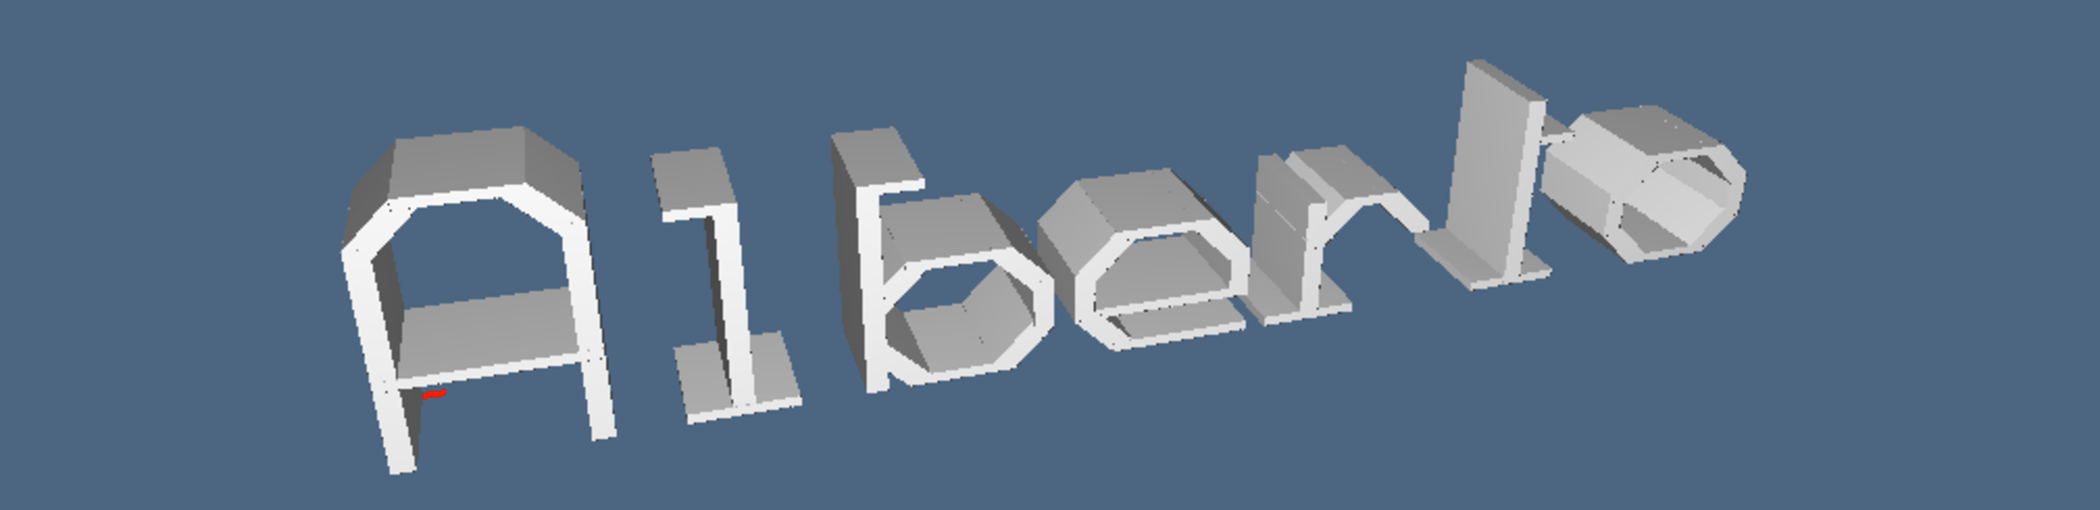
\includegraphics[width=0.8\linewidth]{figs/alberto0a}

\begin{python}
obj = PROD([  OFFSET([0.5,0.25])(TEXT("Alberto")) , Q(3) ])
VIEW(obj)
tensor = MAT([[1,0,0,0],[0,1,0.5,0],[0,0,1,0],[0,0,0,1]])
VIEW(tensor(obj))
\end{python}

\vfill
\centering
\includegraphics[width=0.8\linewidth]{figs/alberto1a}

\vfill\flushleft

QUESTION:	what shearing was applied ?

\end{frame}
%---------------------------------------------------------------------- SLIDE -
\section{Composite transformations}
%---------------------------------------------------------------------- SLIDE -
\begin{frame}[fragile]\frametitle{Composite transformations}

by function composition, NO matrix product !!

\vfill
    
\fbox{rotation of $\pi/4$ about the axis for the edge $((1,0,0),(1,0,1))$}

\vfill

\centering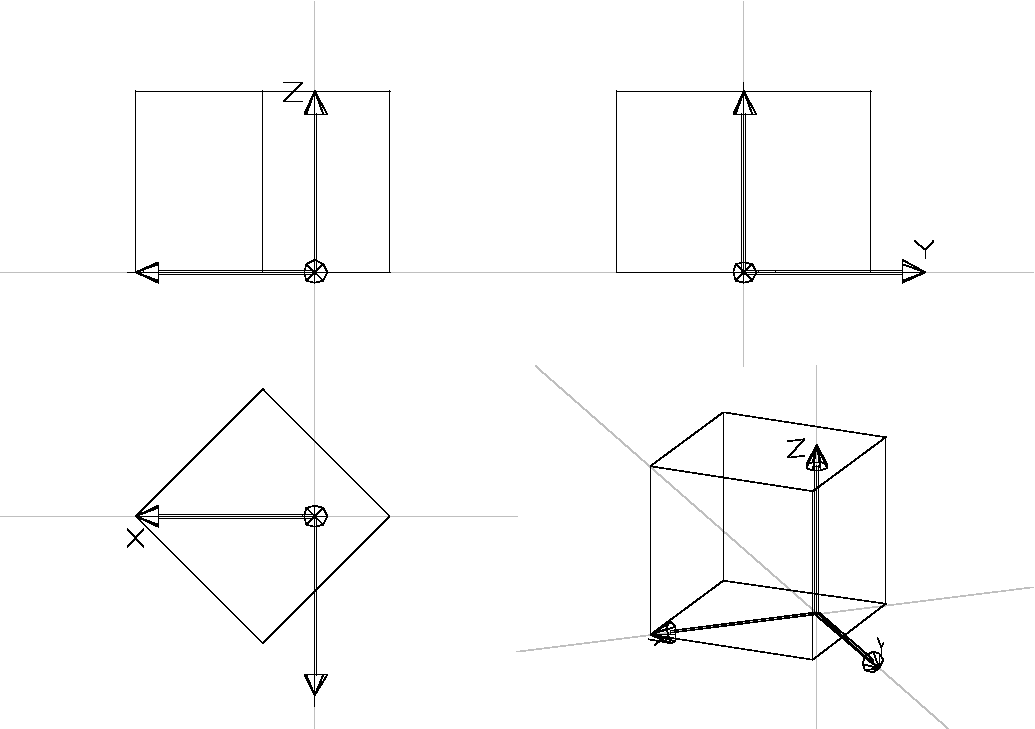
\includegraphics[width=0.6\linewidth]{figs/cube-trt}
\vfill

\begin{python}
 (T:1:1  ~  R:<1,2>:(PI/4)  ~  T:1:-1):(CUBOID:<1,1,1>);
\end{python}


\end{frame}
%---------------------------------------------------------------------- SLIDE -
\begin{frame}\frametitle{Rotation about an affine axis}

\vfill

A more general rotation tensor of ${\E}^3$, with fixed \emph{affine} 1D subspace, i.e.~a line about the origin, is obtained by \alert{composition of transformations} in $\lin\ \R^4$:

\vfill
\[
\T{R}_{xyz}^{*}(\v{n}, \p{p}, \alpha) =
\T{T}_{xyz}(\p{p}-\p{o})\circ \T{R}_{xyz}(\v{n}, \alpha)\circ \T{T}_{xyz}(\p{o}-\p{p})
\]

\vfill

where $\T{R}_{xyz}^{*}(\v{n}, \p{p}, \alpha)$ denotes a \emph{rotation about the $\v{n}$ axis though the point $\p{p}\in{\E}^3$}, and $\p{o}$ is the origin of the Cartesian frame ${\E}^3$.

\vfill

\end{frame}
%---------------------------------------------------------------------- SLIDE -
\begin{frame}\frametitle{Reflection about an affine plane}

\vfill

analogously a reflection $\T{Z}_{xyz}(\v{n},\v{p})$ about to a plane (think to a mirror) with normal $\v{n}$ passing for the point $\v{p}$ need the composition of:

\vfill

\begin{enumerate}

\item a translation $\T{T}_{xyz}(\p{o}-\p{p})$ moving $\v{p}$ to the origin $\v{o}$

\item\vspace{-2mm} a rotation $\T{R}_{xyz}(\v{n}\times\v{e}_3, \alpha)$ moving $\v{n}$ on the axis $\v{e}_3$, with $\alpha =$

\item\vspace{-2mm} a reflection $\T{S}(1,1,-1)$ w.r.t.~a normal coordinate plane

\item\vspace{-2mm} the inverse rotation $\T{R}_{xyz}(\v{n}\times\v{e}_3,-\alpha)$

\item\vspace{-2mm} the inverse translation $\T{T}_{xyz}(\p{p}-\p{o})$
\end{enumerate}

\vfill

\[
\T{Z}_{xyz}(\v{n},\v{p}) =
\]
\[
\T{T}_{xyz}(\p{p}-\p{o})\circ \T{R}_{xyz}(\v{n}\times\v{e}_3,-\alpha) \circ\T{S}(1,1,-1) \T{R}_{xyz}(\v{n}\times\v{e}_3,\alpha)\circ \T{T}_{xyz}(\p{o}-\p{p})
\]


\end{frame}
%---------------------------------------------------------------------- SLIDE -
\begin{frame}\frametitle{Uniform scaling} 
\framesubtitle{definition} \small

\vfill

A uniform scaling $\T{S}_{xyz}(a,a,a)$ is represented by a matrix $(s_{ij})\in\R^{4}_{4}$, different from the identity $4\times 4$ only  by $s_{44}$:
\[
\T{S}_{xyz}(a,a,a) \equiv \mat{
1 & 0 & 0 & 0\\
0 & 1 & 0 & 0\\
0 & 0 & 1 & 0\\
0 & 0 & 0 & 1\over a
}
\]

\vfill

it is easy to verify that:
\[
p^* =
\mat{
1 & 0 & 0 & 0\\
0 & 1 & 0 & 0\\
0 & 0 & 1 & 0\\
0 & 0 & 0 & 1\over a
}
\vet{ x \\ y \\ z \\ 1}
=
\vet{ x \\ y \\ z \\ 1\over a}
=
\vet{ ax \\ ay \\ az \\ 1}
\]

\vfill

\end{frame}

%---------------------------------------------------------------------- SLIDE -
\section{Properties of affine tensors}
%---------------------------------------------------------------------- SLIDE -
\begin{frame}\frametitle{Structure of an affine tensor}

\vfill

The affine transformations of ${\E}^3$, represented in homogeneous coordinates by real matrices $4\times 4$, have the structure:

\[
\T{Z} = \mat{
\T{Q}~ & \v{m} \\
\T{0}^T &  a
}
\]

\vfill

\begin{itemize}
\item 
where $\T{Q}$ is an invertible matrix $3\times 3$

\item \vspace{-2mm}
if $\v{m} \not=
\v{0}$, then $\T{Z}$ has a translation component 

\item \vspace{-2mm}
if $a \not=1$, then we say that $\T{Z}$ is \emph{non normalised}.  In this case it contains a uniform scaling  with parameter $1\over a$.
\end{itemize}

\vfill

\end{frame}
%---------------------------------------------------------------------- SLIDE -
\begin{frame}\frametitle{Action of a tensor on covectors}

\vfill

A linear equation of type $ax + by +cz +d = 0$ (Cartesian equation of a plane in $E^3$) can be written as: 
\[
\v{q} \v{p} = 0
\]
where $\v{q}=(a,b,c,d)$ e $\v{p}=(x,y,z,1)^T$

\vfill
what is the \alert{action of an affine tensor} $\T{M}$ on the affine plane?
We know that it changes lines to lines and planes to planes, ergo

\[
\v{q}^*  \v{p}^* = \v{q}\T{Q}  \T{M}\v{p} = 0
\]
ovvero
\[
\v{q}\T{Q}  \T{M}\v{p} = \v{q}  \v{p}
\]
so $\T{Q} \T{M} = \T{I}$, and hence, for the unknown tensor $\T{Q}$  to be applied to covectors we have: \fbox{$\T{Q} = \T{M}^{-1}$}


\vfill

\end{frame}
%---------------------------------------------------------------------- SLIDE -
\begin{frame}
\frametitle{Properties of tensors}
\framesubtitle{composition or product ??}

\vfill

When a succession of tensors $\T{Q}_1, \T{Q}_2, \ldots, \T{Q}_n$ is applied to a point $\p{p}$, we can write either 

\vfill

\[
\p{p}^* =  (\T{Q}_n\circ \cdots\circ \T{Q}_2\circ \T{Q}_1) (\p{p}),
\]
or
\[
\p{p}^* =  \T{Q}_n\ \cdots\ \T{Q}_2\ \T{Q}_1\ \p{p},
\]

\vfill

depending on the meaning (tensor or matrix) of $\T{Q}_i$ symbol.

\vfill

\end{frame}
%---------------------------------------------------------------------- SLIDE -
\begin{frame}\frametitle{Properties of tensors}
\framesubtitle{Associativity}

\vfill

Both the tensor composition and the product of matrices are associative operations (left-and or right-hand)

\vfill

\[
 (\T{Q}_3\circ \T{Q}_2)\circ \T{Q}_1
= \T{Q}_3\circ (\T{Q}_2\circ \T{Q}_1)
=  \T{Q}_3\circ \T{Q}_2 \circ \T{Q}_1
\]

\[
(\T{Q}_3 \T{Q}_2)\ \T{Q}_1
= \T{Q}_3\ (\T{Q}_2 \T{Q}_1)
= \T{Q}_3 \T{Q}_2  \T{Q}_1
\]

\vfill

The use of parentheses is hence not needed to specify the order of operations
\end{frame}

%---------------------------------------------------------------------- SLIDE -
\begin{frame}\frametitle{Properties of tensors}
\framesubtitle{Non commutativity}

\vfill
 
In general,  the composition of tensors  and the product of matrices are not commutative:
\[
\T{Q}_1\circ \T{Q}_2 \not= \T{Q}_2\circ \T{Q}_1 \quad\mbox{e}\quad
\T{Q}_1 \T{Q}_2 \not= \T{Q}_2 \T{Q}_1,
\]

\vfill

But there are important exceptions to this rule:\\
e.g., are \emph{commutative} (the list is not complete):

\vfill

\begin{enumerate}
    \item the composition (product) of rotations about the same axes;
    \item\vspace{-2mm} the composition (product) of translations;
    \item\vspace{-2mm} the composition (product) of scalings;
    \item\vspace{-2mm} the composition (product) of rotations and uniform scalings;.
\end{enumerate}

\end{frame}
%---------------------------------------------------------------------- SLIDE -
\begin{frame}\frametitle{Properties of tensors}
\framesubtitle{Composition}

\vfill
Rotation and translation tensors \emph{additive composability}:

\[
\T{T}_{xy}(m_1,n_1)\circ \T{T}_{xy}(m_2,n_2) = \T{T}_{xy}(m_1+m_2,n_1+n_2),
\]

\[
\T{R}_{xy}(\alpha_1)\circ \T{R}_{xy}(\alpha_2)= \T{R}_{xy}(\alpha_1+\alpha_2)
\]
\vfill

conversely, scaling tensors have \emph{multiplicative composability}:

\[
\T{S}_{xy}(a_1,b_1)\circ \T{S}_{xy}(a_2,b_2)= \T{S}_{xy}(a_1 a_2,b_1 b_2)
\]

\vfill

\end{frame}
%---------------------------------------------------------------------- SLIDE -
\begin{frame}\frametitle{Properties of tensors}
\framesubtitle{Inverse}

\vfill

It follows, for inverse transformations:

\vfill

\[
\left(\T{T}_{xy}(m,n)\right)^{-1} = \T{T}_{xy}(-m,-n)
\]

\vfill
\[
\left(\T{R}_{xy}(\alpha)\right)^{-1} = \T{R}_{xy}(-\alpha)
\]

\vfill
\[
\left(\T{S}_{xy}(a,b)\right)^{-1} = \T{S}\left({1\over a}, {1\over b}\right)
\]

\vfill

\end{frame}
%---------------------------------------------------------------------- SLIDE -
\begin{frame}[fragile]
\frametitle{Examples}
\framesubtitle{2D/3D Clock model}

\vfill

Circular \texttt{background},  $12$ \texttt{ticks} of hours, and 
\texttt{hour} and \texttt{minute} hands,  given in their local coordinate systems

\vfill

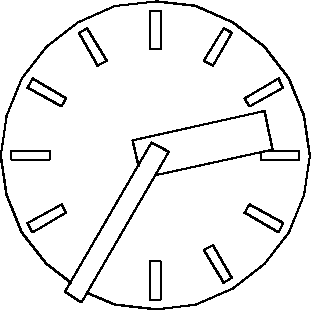
\includegraphics[width=0.2\linewidth]{figs/clock1}
\hspace{1.5cm}

\includegraphics[width=0.2\linewidth]{figs/clock2}
\hspace{1.5cm}

\includegraphics[width=0.18\linewidth]{figs/clock3}

\vfill

\begin{python}
background = COLOR(RED)(CIRCLE(0.8)([48,1]))
minute = T([1,2])([-0.05,-0.05])(CUBOID([0.9,0.1])) 
hour = T([1,2])([-0.1,-0.1])(CUBOID([0.7,0.2]))
tick = T([1,2])([-0.025,0.55])(CUBOID([0.05,0.2])) 
ticks = STRUCT(NN(12)([ tick, R([1,2])(PI/6) ]))
\end{python}


\end{frame}
%---------------------------------------------------------------------- SLIDE -
\begin{frame}[fragile]\frametitle{Examples}
\framesubtitle{2D/3D Clock model}

\vfill


\begin{python}
def clock2D (h,m):
    return STRUCT([ background, ticks,
	    R([1,2])( PI/2 - (h + m/60)*PI/6 )(hour),
	    R([1,2])( PI/2 - m*PI/30 )(minute) ])
\end{python}


\begin{python}
def clock3D (h,m):
    return STRUCT([  
    	COLOR(RED)(PROD([ background, Q(0.2) ])),
    	T(3)(0.2)(PROD([ ticks, Q(0.01) ])), T(3)(0.2),
    	R([1,2])( PI/2 - (h + m/60.)*PI/6 )(PROD([ hour, Q(0.03) ])), T(3)(0.03),
    	R([1,2])( PI/2 - m*PI/30 )(PROD([ minute, Q(0.03) ])) ])
\end{python}

\vfill

\end{frame}
%---------------------------------------------------------------------- SLIDE -
\begin{frame}[fragile]\frametitle{Examples}
\framesubtitle{2D/3D Clock model}

\vfill\centering

   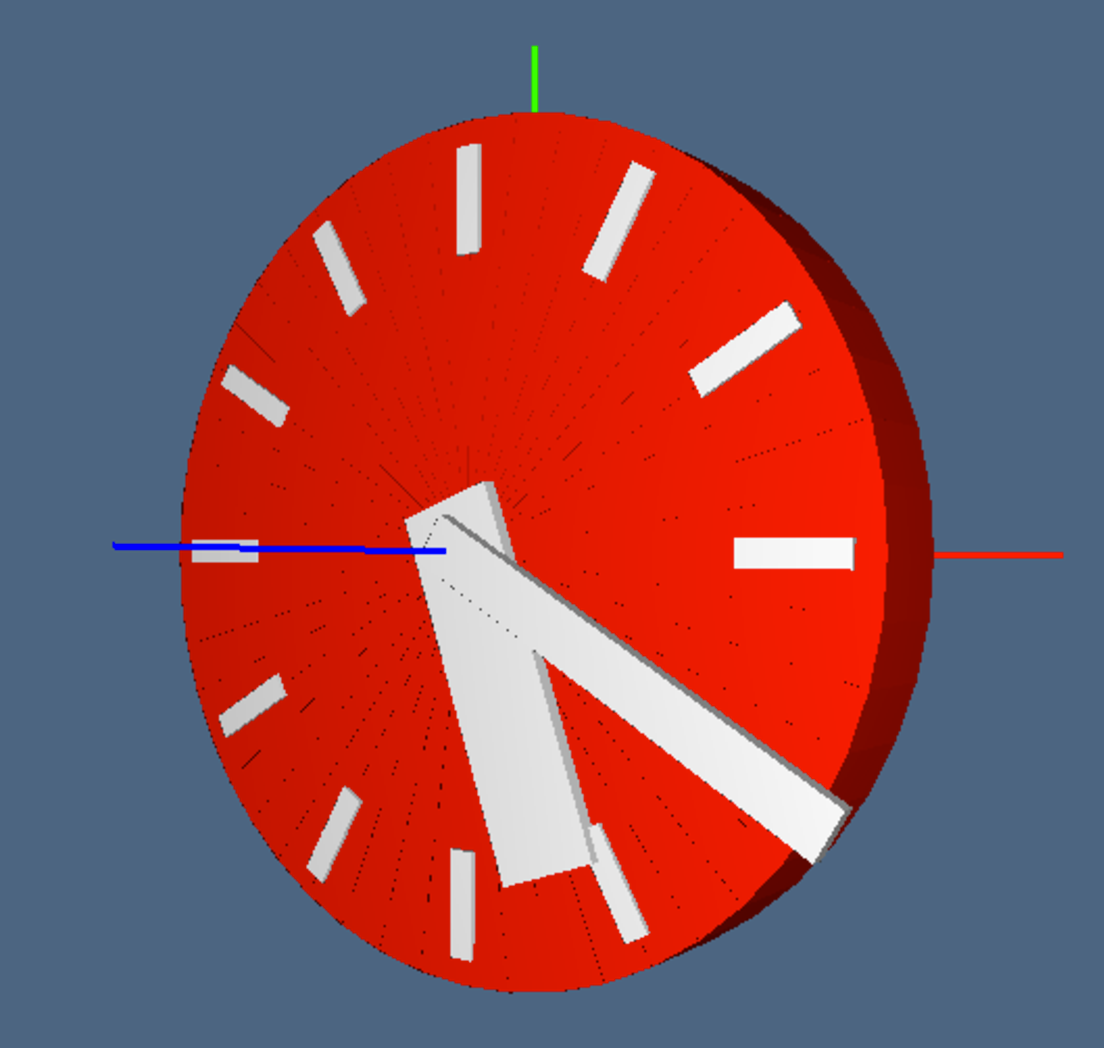
\includegraphics[width=2in]{figs/newclock} 

\begin{python}
VIEW(clock3D(5,20))
\end{python}


\end{frame}
%---------------------------------------------------------------------
%---------------------------------------------------------------------- SLIDE -
\end{document}

